\documentclass{beamer}\usepackage[]{graphicx}\usepackage[]{color}
%% maxwidth is the original width if it is less than linewidth
%% otherwise use linewidth (to make sure the graphics do not exceed the margin)
\makeatletter
\def\maxwidth{ %
  \ifdim\Gin@nat@width>\linewidth
    \linewidth
  \else
    \Gin@nat@width
  \fi
}
\makeatother

\definecolor{fgcolor}{rgb}{0.345, 0.345, 0.345}
\newcommand{\hlnum}[1]{\textcolor[rgb]{0.686,0.059,0.569}{#1}}%
\newcommand{\hlstr}[1]{\textcolor[rgb]{0.192,0.494,0.8}{#1}}%
\newcommand{\hlcom}[1]{\textcolor[rgb]{0.678,0.584,0.686}{\textit{#1}}}%
\newcommand{\hlopt}[1]{\textcolor[rgb]{0,0,0}{#1}}%
\newcommand{\hlstd}[1]{\textcolor[rgb]{0.345,0.345,0.345}{#1}}%
\newcommand{\hlkwa}[1]{\textcolor[rgb]{0.161,0.373,0.58}{\textbf{#1}}}%
\newcommand{\hlkwb}[1]{\textcolor[rgb]{0.69,0.353,0.396}{#1}}%
\newcommand{\hlkwc}[1]{\textcolor[rgb]{0.333,0.667,0.333}{#1}}%
\newcommand{\hlkwd}[1]{\textcolor[rgb]{0.737,0.353,0.396}{\textbf{#1}}}%
\let\hlipl\hlkwb

\usepackage{framed}
\makeatletter
\newenvironment{kframe}{%
 \def\at@end@of@kframe{}%
 \ifinner\ifhmode%
  \def\at@end@of@kframe{\end{minipage}}%
  \begin{minipage}{\columnwidth}%
 \fi\fi%
 \def\FrameCommand##1{\hskip\@totalleftmargin \hskip-\fboxsep
 \colorbox{shadecolor}{##1}\hskip-\fboxsep
     % There is no \\@totalrightmargin, so:
     \hskip-\linewidth \hskip-\@totalleftmargin \hskip\columnwidth}%
 \MakeFramed {\advance\hsize-\width
   \@totalleftmargin\z@ \linewidth\hsize
   \@setminipage}}%
 {\par\unskip\endMakeFramed%
 \at@end@of@kframe}
\makeatother

\definecolor{shadecolor}{rgb}{.97, .97, .97}
\definecolor{messagecolor}{rgb}{0, 0, 0}
\definecolor{warningcolor}{rgb}{1, 0, 1}
\definecolor{errorcolor}{rgb}{1, 0, 0}
\newenvironment{knitrout}{}{} % an empty environment to be redefined in TeX

\usepackage{alltt}

\mode<presentation>
{
 \usetheme{AnnArbor}
 \usecolortheme{crane}
}
\setbeamertemplate{navigation symbols}{}
\usepackage[english]{babel}
\usepackage{times}
\usepackage[T1]{fontenc}
\usepackage[applemac]{inputenc}
\usepackage{amsmath}


\setbeamerfont{caption}{size=\scriptsize}
\setbeamertemplate{caption}{\raggedright\insertcaption\par}
\usepackage{hyperref}  
\hypersetup{colorlinks=true,allcolors=blue}

\title[RNA-seq]{Introduction to RNA sequencing}
\subtitle{Bioinformatics perspective}
\author[Olga]{Olga Dethlefsen}
\institute[NBIS]{NBIS, National Bioinformatics Infrastructure Sweden\\}
\date[November 2017]{November 2017}


\logo{%
  \makebox[0.95\paperwidth]{%
    
\includegraphics[height=1cm,keepaspectratio]{Logos/nbislogo-orange.png}%
    \hfill%
    
\includegraphics[height=1cm, keepaspectratio]{Logos/SciLifeLab-logo.jpg}%
  }%
}

\useinnertheme{rectangles}

\AtBeginSection[]{
  \begin{frame}
  \vfill
  \centering
  \begin{beamercolorbox}[sep=8pt,center,shadow=true,rounded=true]{title}
    \usebeamerfont{title}\insertsectionhead\par%
  \end{beamercolorbox}
  \vfill
  \end{frame}
}

\usepackage[style=british]{csquotes}
\usepackage{csquotes}
\IfFileExists{upquote.sty}{\usepackage{upquote}}{}
\begin{document}

\begin{frame}
\titlepage
\end{frame}
\logo{}


% Outline
% Why sequence transcriptome
% From RNA to sequence
% Reference based analysis
  % Entire pipeline incl. GO / REACTOME pathways
% What about de-novo assmebly of transcripotmes
% What about scRNA-seq
% Summary
% Tutorial



\begin{frame}
\begin{block}{Outline}
\begin{itemize}
  \item Why sequence transcriptome?
  \item From RNA to sequence
  \item The most common way: reference based analysis pipeline
  \item What about de-novo assembly of transcriptomes?
  \item And what about scRNA-seq?
  \item Summary
  \item Introduction to exercises
 \end{itemize}
\end{block}
\end{frame}

\section{Why sequence transcriptome?}

%\usebackgroundtemplate{%
 % 
\includegraphics[width=\paperwidth,height=\paperheight]{Logos/20x15cm}} 
 
% Transcriptome: overview figure
\begin{frame}
\begin{center}
\begin{figure}
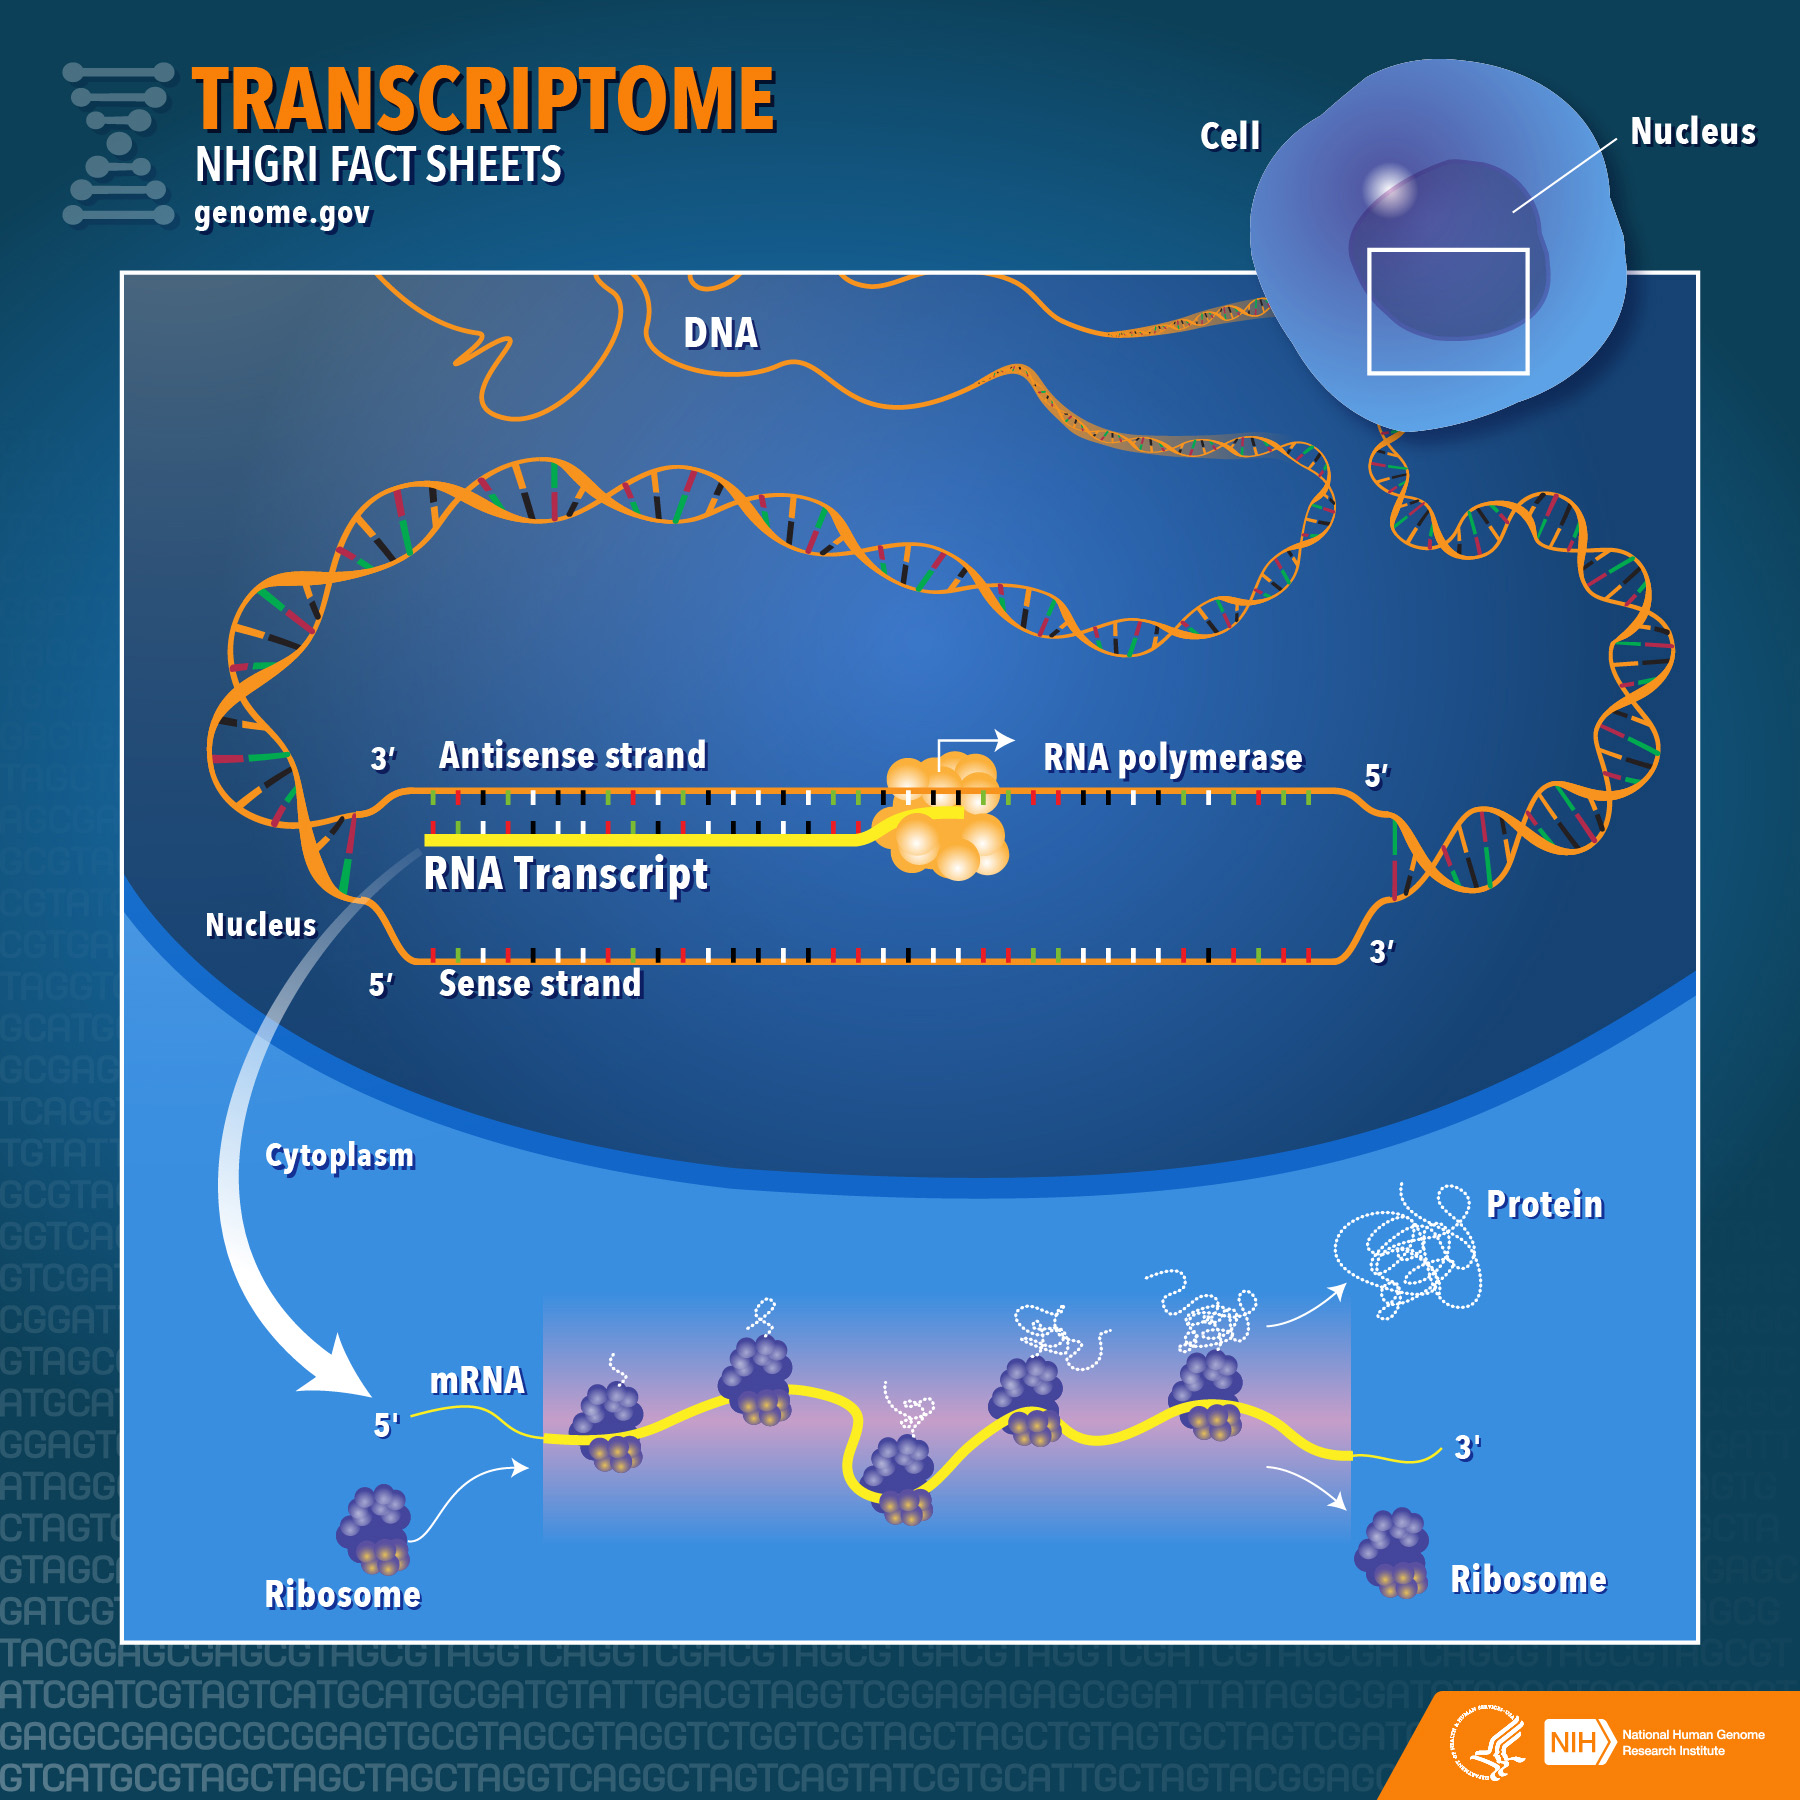
\includegraphics[height=8cm]{Images/transcriptome.jpg}
%\caption{Figure: Simplified scRNA-seq workflow [adopted from \href{http://hemberg-lab.github.io/]}{http://hemberg-lab.github.io/}}
\end{figure}
\end{center}
\end{frame}


% Why study transcriptome: quote
\begin{frame}
\begin{displayquote}
An RNA sequence mirrors the sequence of the DNA from which it was transcribed.
\end{displayquote}
\begin{displayquote}
Consequently, by analyzing transcriptome we can determine when and where each gene is turned on or off in the cells and tissues of an organism.
\end{displayquote}
\end{frame}

% Why study transcriptome: what can a transcriptome tell us about?
\begin{frame}
\begin{block}{What can a transcriptome tell us about?}
\begin{itemize}
\item gene sequences in genomes
\item gene functions
\item gene activity / gene expression
\item isoforms and allelic expression
\item fusion transcripts and novel transcripts
\item SNPs in genes
\item co-expression of genes 
\item cell-to-cell heterogeneity (scRNA-seq)
\end{itemize}
\end{block}
\end{frame}

% Why study transcriptome: what makes RNA-seq different to genome sequencing
\begin{frame}
Transcriptomes are: \newline \newline
\begin{displayquote}
dynamic, that is not the same over tissues and time points
\end{displayquote}
\begin{displayquote}
directly derived from functional genomics elements, that is mostly protein-coding genes, providing a useful functionally relevant subset of the genome, translating into smaller sequence space
\end{displayquote}
\end{frame}

% Why study transcriptome: overview
\begin{frame}
\begin{block}{Overview}
\begin{itemize}
\item \color{blue} Experimental design \color{black}(biology, medicine, statistics)
\item \color{blue} RNA extraction \color{black}(biology, biotechnology)
\item \color{blue} Library preparation (\color{black}biology, biotechnology)
\item \color{blue} High throughput sequencing \color{black}(engineering, biology, chemistry, biotechnology, bioinformatics)
\item \color{red} Data processing \color{black} (bioinformatics)
\item \color{red} Data analysis \color{black} (bioinformatics \& biostatistics)
\end{itemize}
\end{block}
\end{frame}


%% From RNA to sequence
\section{From RNA to sequence}

%% From RNA to sequence: workflow v01
\begin{frame}
\begin{center}
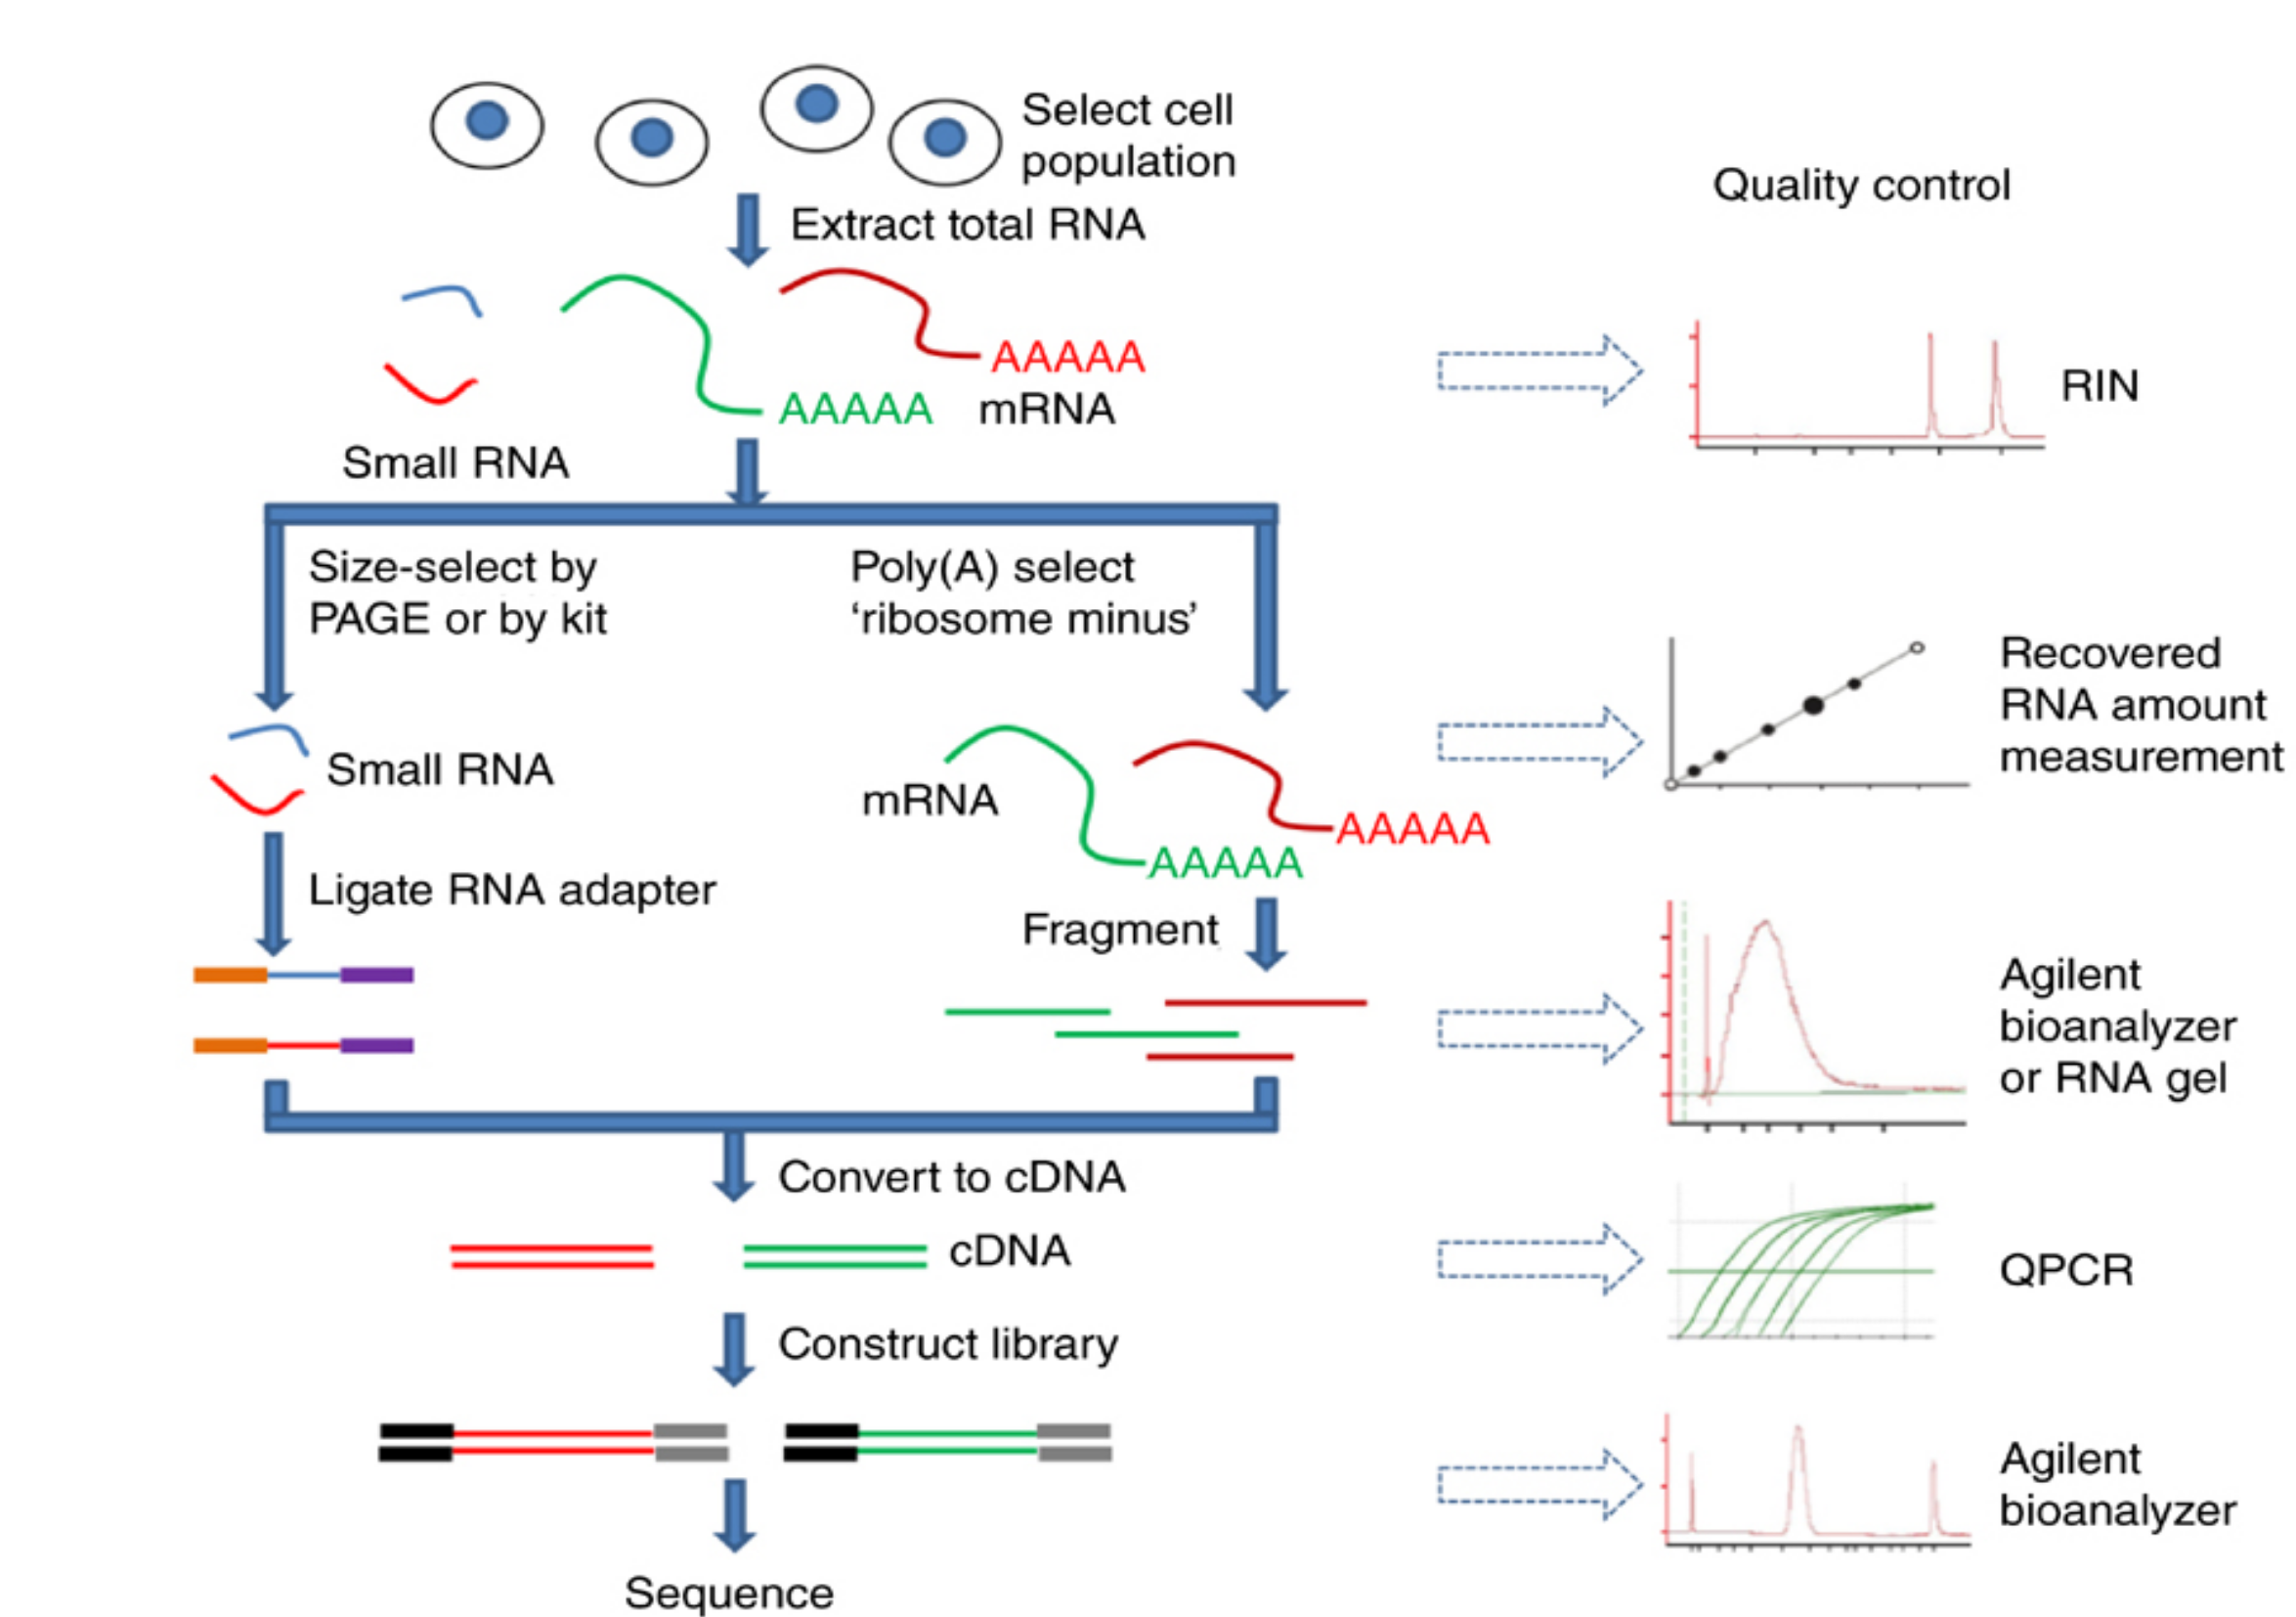
\includegraphics[height=8cm]{Images/RNA2seq.jpg}
\end{center}
\end{frame}

%% From RNA to sequence: workflow v02
\begin{frame}
\begin{center}
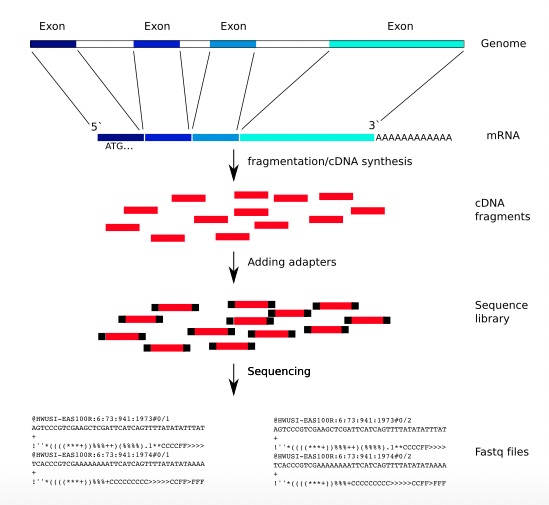
\includegraphics[height=8cm]{Images/RNA2seq2}
\end{center}
\end{frame}

%% From RNA to sequence: .fastq
\begin{frame}
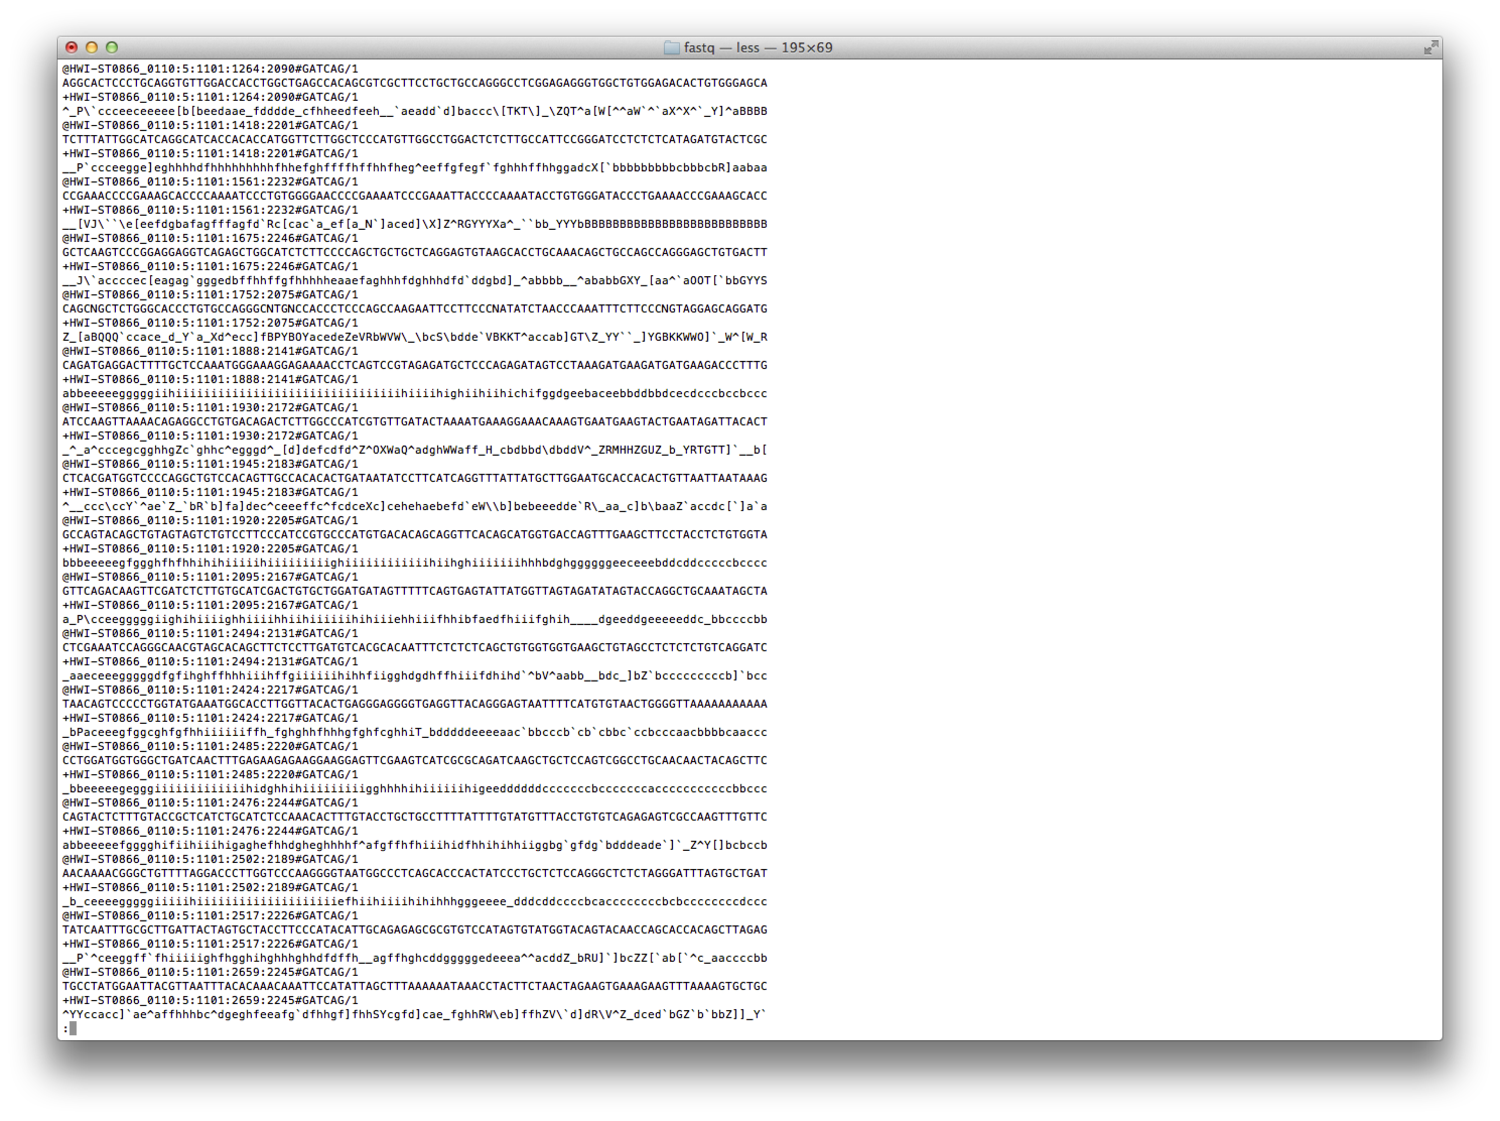
\includegraphics[width=15cm]{Images/fastqless.pdf}
\end{frame}

%% From RNA to sequence: .fastq
\begin{frame}
\begin{block}{.fastq}
@MISEQ:233:000000000-AGJP2:1:1101:15260:1358
CTGTAAATTGCCTGACTTGCTAATTGTGATTAACTTAGTTT \newline
+ \newline
BBBBBFFFFFFFGGGGGGGGGGHFFFHGHHGFFHHHHHAG
\end{block}
\begin{itemize}
\item Line1: \pause begins with a '@' character and is followed by a sequence identifier and an optional description 
\item Line2: \pause is the raw sequence letters 
\item Line3: \pause begins with a '+' character and is optionally followed by the same sequence identifier (and any description) again 
\item Line4: \pause encodes the quality values for the sequence in Line 2, and must contain the same number of symbols as letters in the sequence
\end{itemize}
\end{frame}

% Understanding sequencing output (quality explanation)
\begin{frame}
\begin{columns}
\column{6cm}
\centering
\begin{block}{Phred Quality Score}
\begin{itemize}
\item Q = -10 x log P
\item where:
\begin{itemize}
\item P, probability of base calling being incorrect
\item High Q = high probability of the base being correct
\end{itemize}
\end{itemize}
\end{block}
\column{6cm}
\centering
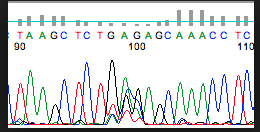
\includegraphics[width=5cm]{Images/phred.png}
\end{columns}
\begin{itemize}
\item A Phred quality score of 10 to a base means that the base is called incorrectly in 1 out of...\pause 10 times.
\item A Phred quality score of 20 to a base, means that the base is called incorrectly in 1 out of...\pause 100 times.
\item A Phred quality score of 30 to a base, means that the base is called incorrectly in 1 out of...\pause 1000 times etc...
\end{itemize}
\end{frame}


% Understanding sequencing output: SE vs PE
\begin{frame}
\begin{block}{PE, paired-end}
\begin{itemize}
\item Two .fastq files are created per sequenced library
\item The order of reads in files is identical and naming of reads is the same with the exception of the end information
\item The way of naming reads are changing over time so the read names depend on software version
\end{itemize}
\end{block}
\vspace{8mm}
\centering
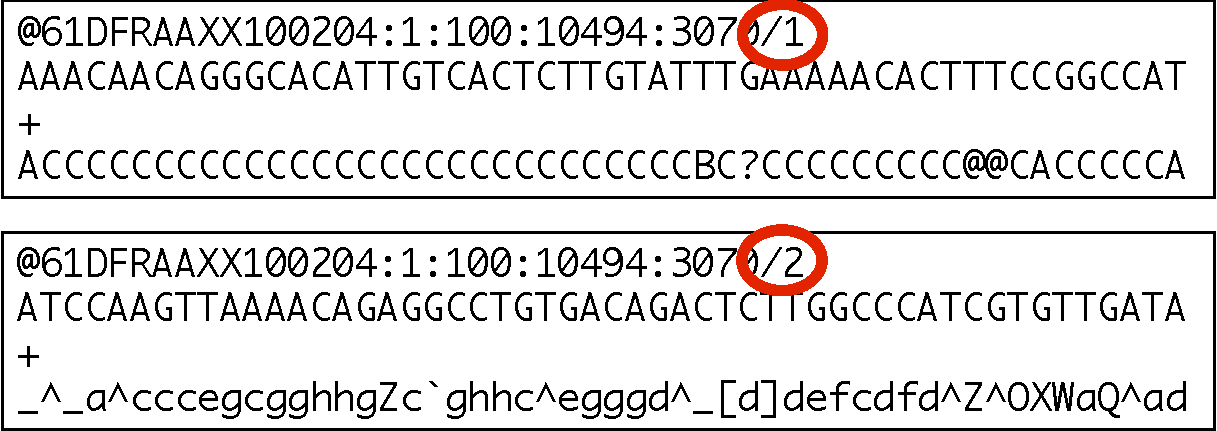
\includegraphics[width=8cm]{Images/fastqPE.pdf}
\end{frame}

% Understanding sequencing output: Strandness
\begin{frame}
\footnotesize
\begin{columns}
\begin{column}{0.48\textwidth}
SE
\begin{itemize}
  \item F: the single read is in the sense (F, forward) orientation
  \item R: the single read is in the antisense (R, reverse) orientation
\end{itemize}
PE
\begin{itemize}
\item RF: first read (/1) is sequenced as anti-sense (R) \& second read (/2) is in the sense strand (F)
\item FR: first read (/1) is sequenced as sense (F) \& second read (/2) is in the antisense strand (R)
\end{itemize}
\end{column}
\begin{column}{0.48\textwidth}
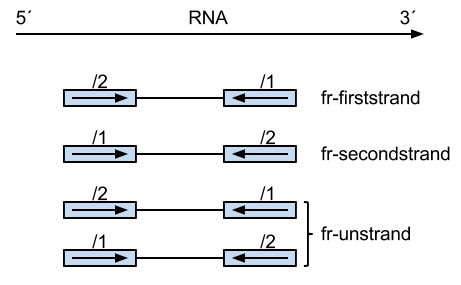
\includegraphics[width=5cm]{Images/Stranded.png}
\end{column}
\end{columns}
\end{frame}

% Reference based data analysis pipeline
\section{Reference based data analysis pipeline}

% Reference based data analysis pipeline: overview figure
\begin{frame}
\centering
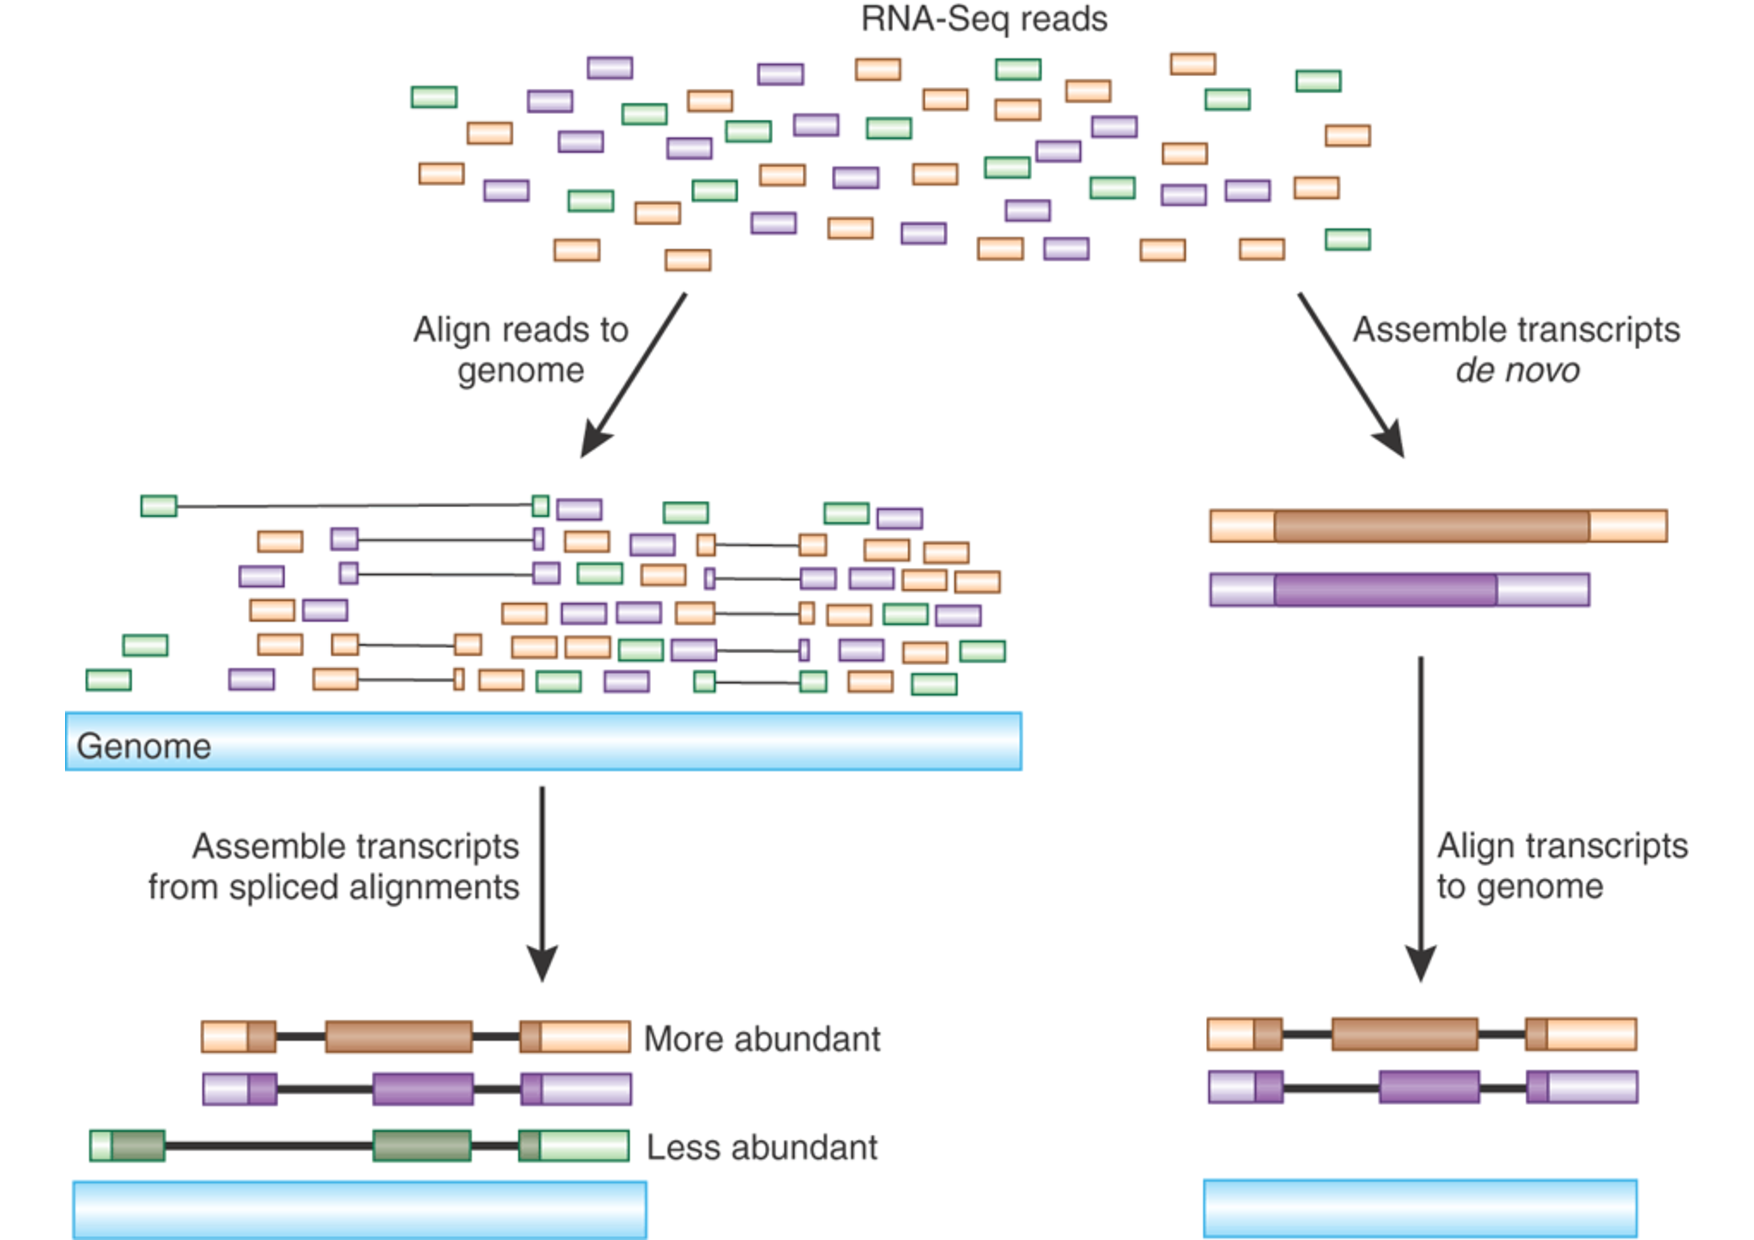
\includegraphics[width=9cm]{Images/workflows.pdf}
 % \\{\tiny{Haas \& Zody (2010), Nature Biotechnology 28, 421--423}}
\end{frame}

% Reference based data analysis pipeline: main steps
\begin{frame}
\begin{block}{Main steps}
\begin{itemize}
  \item Initial processing incl. QC
  \item Aligning reads to reference genome
  \item Counting reads
  \item Differential gene expression
  \item Annotations of transcripts
\end{itemize}
\end{block}
\end{frame}

% Reference based data analysis pipeline: filtering
\begin{frame}
\frametitle{Initial processing incl. QC}
\footnotesize
\begin{columns}
\begin{column}{0.38\textwidth}
\begin{itemize}
\item Demultiplex by index or barcode
\item Remove adapter sequences
\item Trim reads by quality
\item Discard reads by quality/ambiguity
\end{itemize}
\end{column}
\begin{column}{0.58\textwidth}
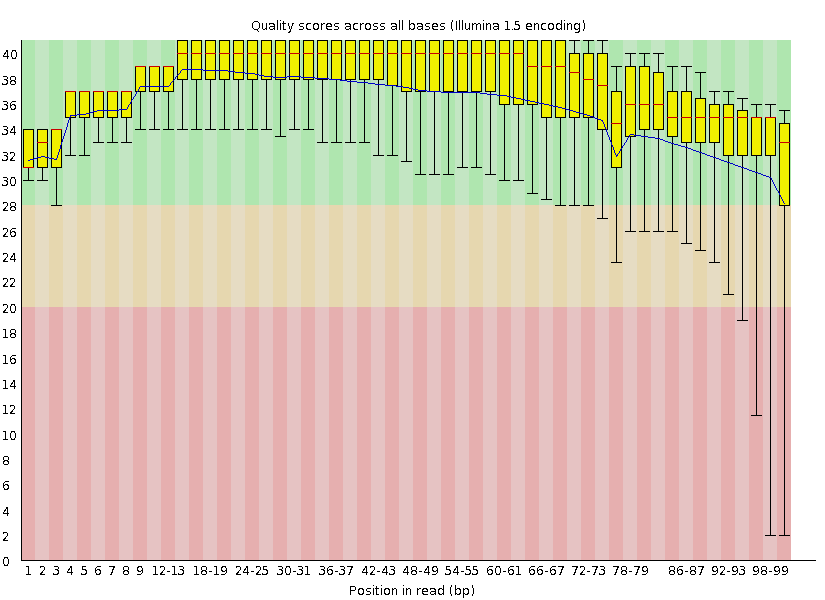
\includegraphics[width=7cm]{Images/fastq_qc_good.png}
\end{column}
\end{columns}
\vspace{5mm}
\begin{block}{Available tools}
FastQC, PRINSEQ, TRIMMOMATIC, TrimGalore, FastX, Cutadapt
\end{block}
\end{frame}

% Reference based data analysis pipeline: filtering
\begin{frame}
\frametitle{Initial processing incl. QC}
\centering
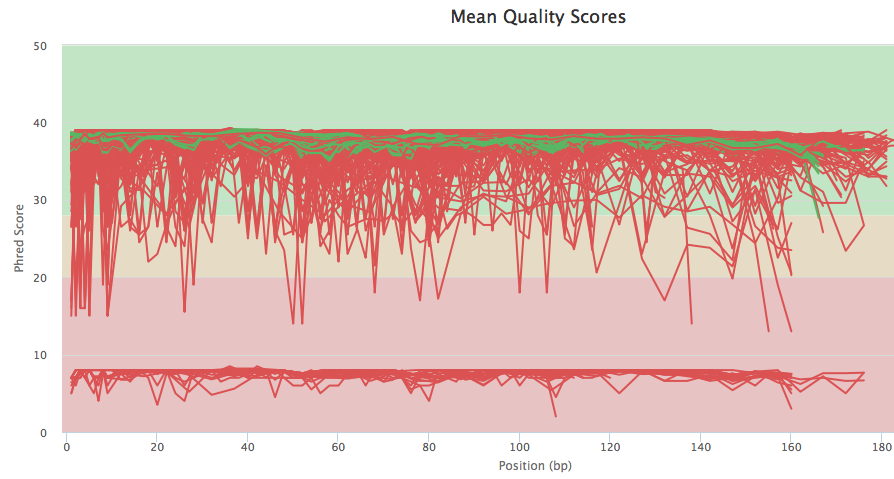
\includegraphics[width=10cm, height=4cm]{Images/fastq_qc_poor.png}
\begin{itemize}
\footnotesize
\item filtering reads for quality score, e.g. with avg. quality below 20 defined within 4-base wide sliding window
\item filtering reads for read length, e.g. reads shorter than 36 bases
\item removing artificial sequences, e.g. adapters
\end{itemize}
\end{frame}


% Reference based data analysis pipeline: mapping
\begin{frame}
\frametitle{Aligning reads}
\centering
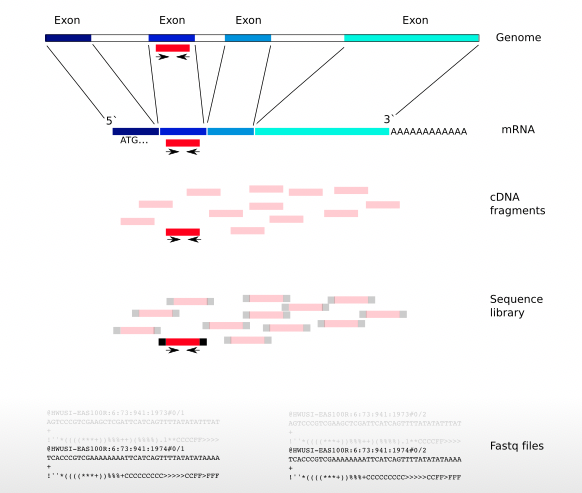
\includegraphics[height=6cm]{Images/map1.png}
\end{frame}

% Reference based data analysis pipeline: mapping
\begin{frame}
\frametitle{Aligning reads}
\centering
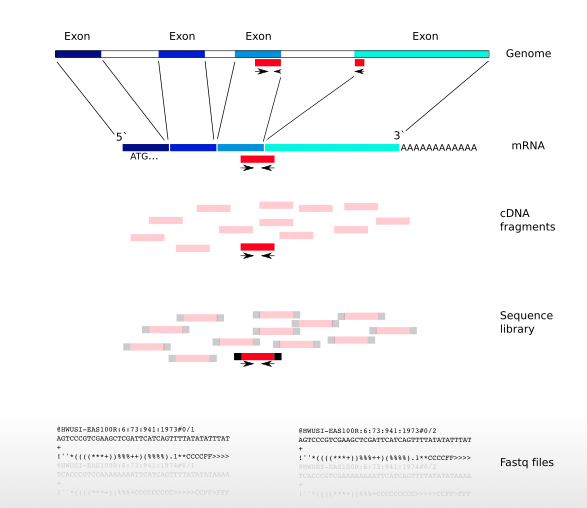
\includegraphics[height=6cm]{Images/map2.png}
\end{frame}

% Reference based data analysis pipeline: mapping aligenrs
\begin{frame}
\frametitle{Aligning reads: mappers}
\footnotesize
\begin{itemize}
  \item important to use mappers allowing for a read to be "split" between distant regions of the reference in the event that the read spans two exons
  \item lots of different aligners exists based on various algorithms e.g. brute force comparison, Burrows-Wheeler Transform, Smith-Waterman, Suffix tree
  \item usually there is a trade-off between speed versus accuracy and sensitivity
  \item usually the "biggest differece" is with default settings, most mappers will allow to optimise settings
  \item perfomance vary by genome complexity
\end{itemize}

\textit{A good read: Barruzo et. al. Nature Methods 14, (2017) \href{Simulation-based comprehensive benchmarking of RNA-seq aligners}{https://www.nature.com/articles/nmeth.4106}}

\vspace{5mm}
\begin{block}{Available tools}
STAR, HISAT, MapSlice2, Subread, TopHat
\end{block}
\end{frame}

% Reference based data analysis pipeline: mapping files
\begin{frame}
\frametitle{Aligning reads: reference files}
.fasta (download reference genome FASTA file)
\newline
\begin{center}
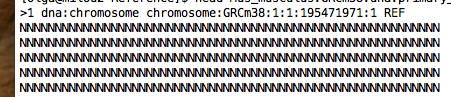
\includegraphics[width=10cm, height=1.5cm]{Images/ref.png}
\end{center}
.gtf (download the corresponding genome annotation in GTF or GFF)
\begin{center}
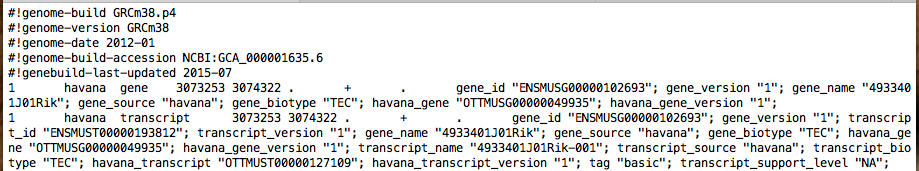
\includegraphics[width=10cm, height=2cm]{Images/ref_annotation.png}
\end{center}
\vspace{5mm}
\begin{block}{Source}
ENSEMBL, NCBI
\end{block}
\end{frame}

% Reference based data analysis pipeline: mapping
\begin{frame}
\frametitle{Aligning reads}
\centering
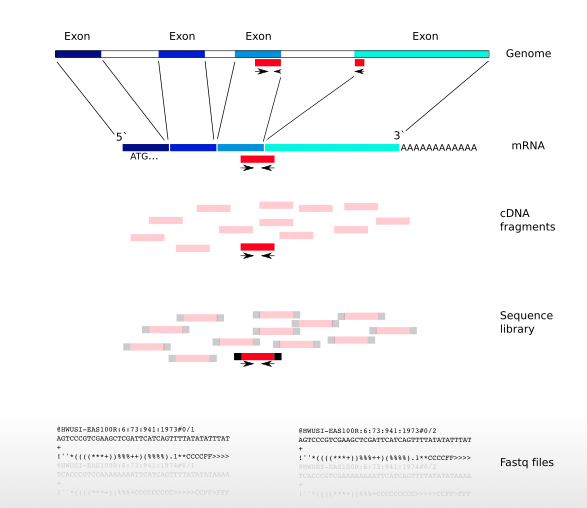
\includegraphics[height=6cm]{Images/map2.png}
\end{frame}

% Reference based data analysis pipeline: mapping QC
\begin{frame}
\frametitle{Aligning reads: QC}
\begin{center}
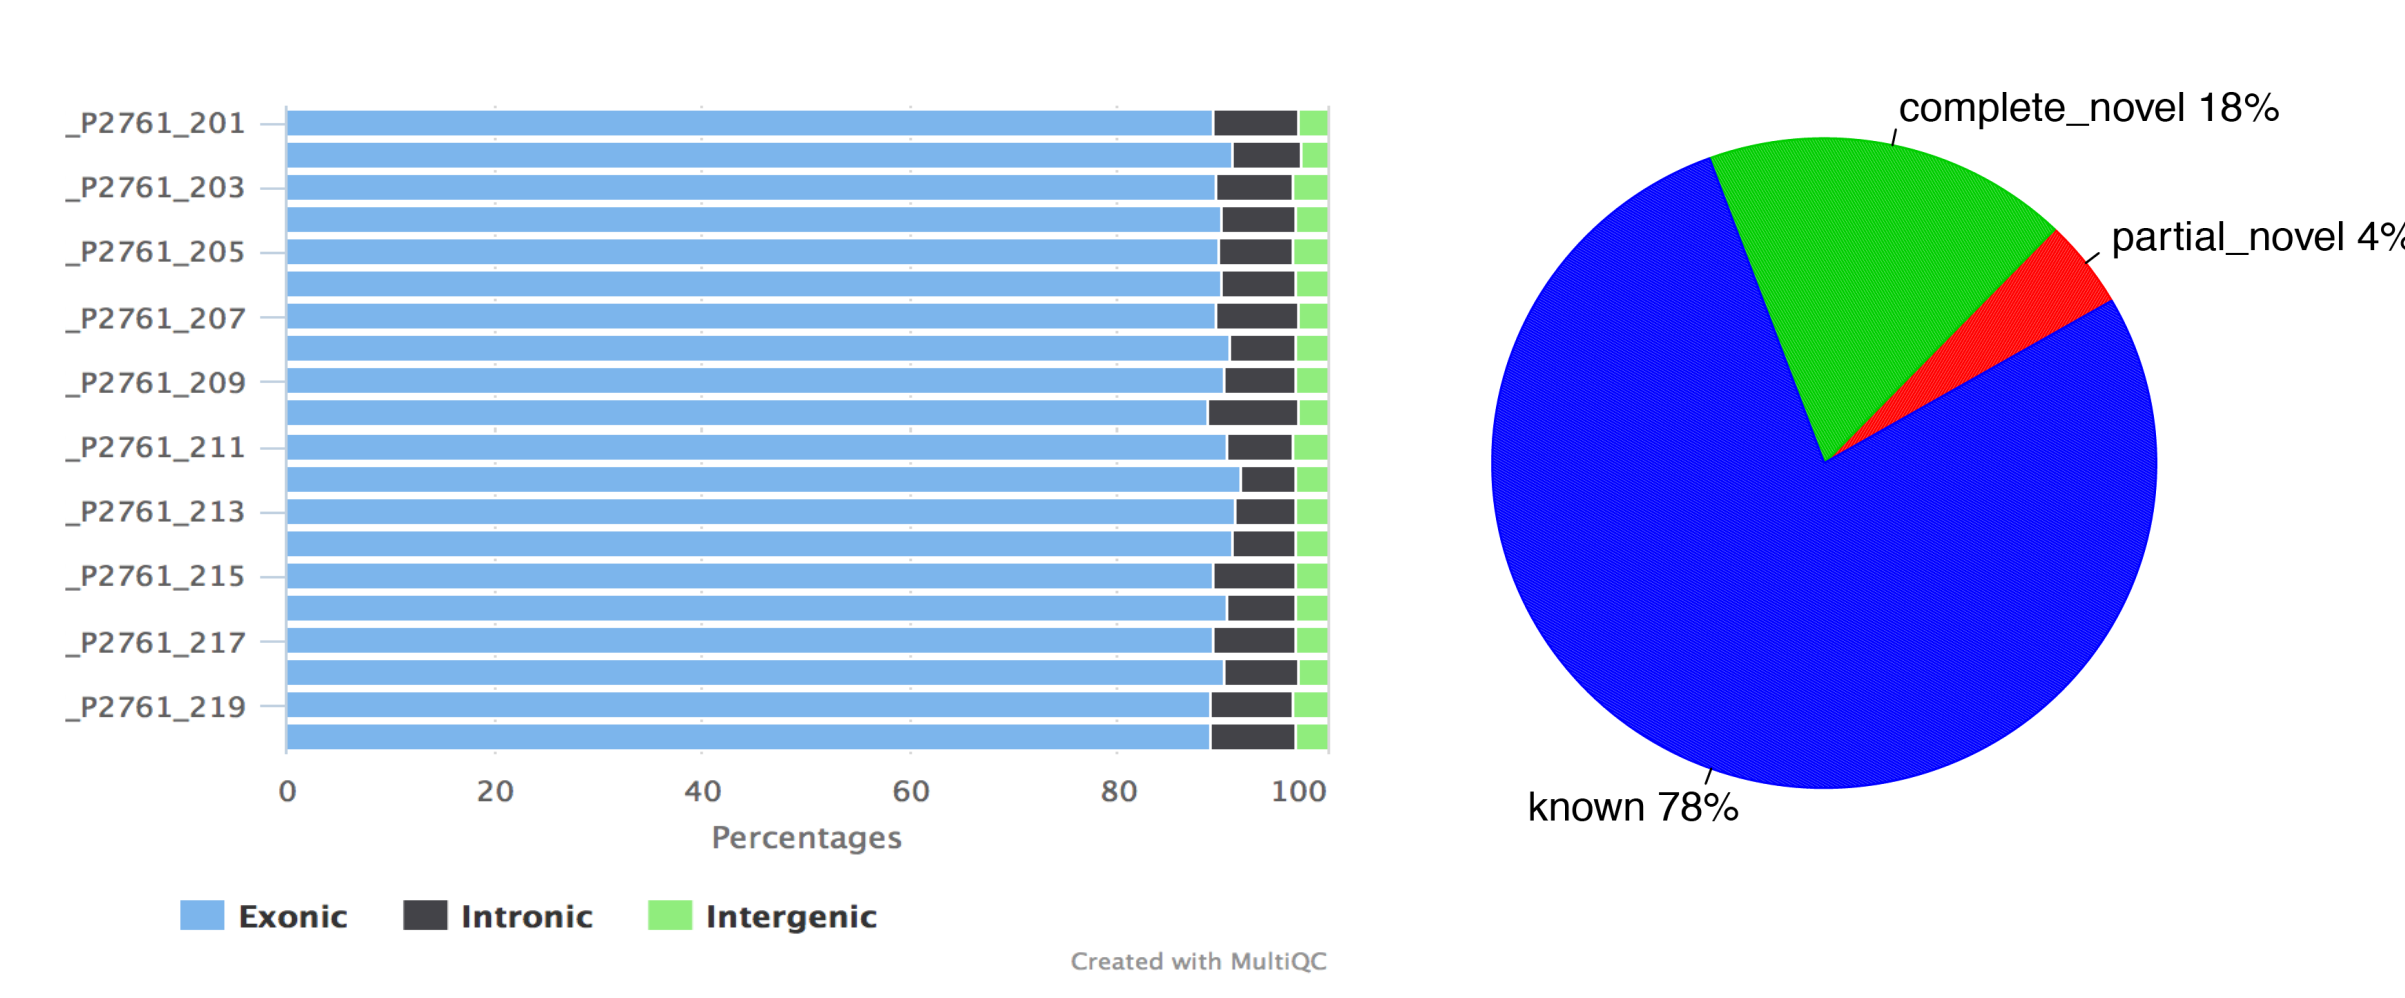
\includegraphics[width=12cm]{Images/map_qual.png}
\end{center}
Post mapping QC, e.g. reads should mostly map to known genes, most splice event should be known and canonical (GU-AG)
\end{frame}


% Reference based data analysis pipeline: counting
\begin{frame}
\frametitle{Counting reads}
\begin{center}
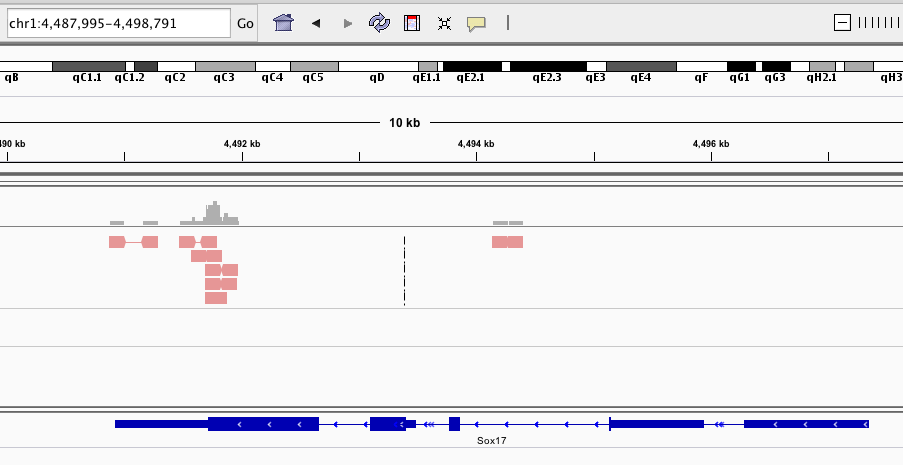
\includegraphics[width=10cm, height=5cm]{Images/counts_IGV.png}
\end{center}
\begin{block}{Available tools}
HTSeq, featureCounts, R
\end{block}
\end{frame}

% Reference based data analysis pipeline: counting
\begin{frame}
\frametitle{Counting reads}
\centering
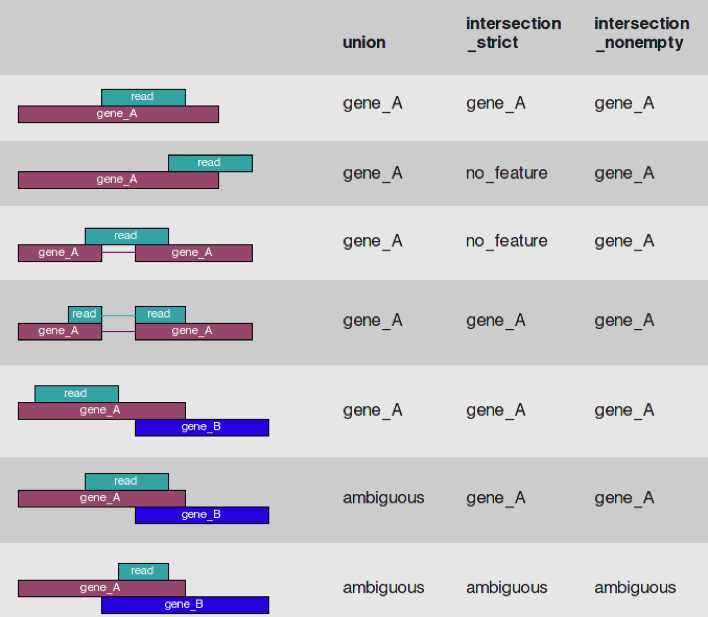
\includegraphics[width=7cm]{Images/counts_HTseq.png}
  \\{\tiny{from: http://www-huber.embl.de/users/anders/HTSeq/doc/count.html}}
\end{frame}

% Reference based data analysis pipeline: counting
\begin{frame}
\frametitle{Counting reads}
\begin{center}
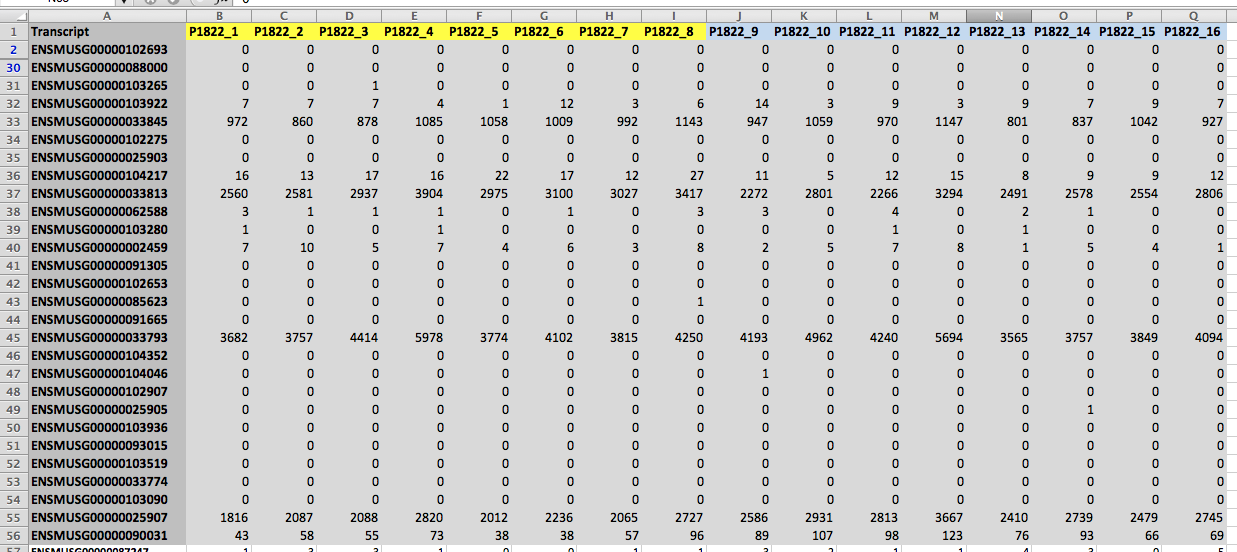
\includegraphics[width=12cm, height=7cm]{Images/counts_table.png}
\end{center}
\end{frame}


% Reference based data analysis pipeline: differential expression
\begin{frame}
\frametitle{Differential gene expression}
Differential expression analysis
\begin{itemize}
\item means taking the normalized read count data \&
\item performing statistical analysis to discover quantitative changes in expression levels between experimental groups. 
\item e.g. to decide whether, for a given gene, an observed difference in read counts is significant, that is, whether it is greater than what would be expected just due to natural random variation.
\item or simply: checking for differences in distributions
\end{itemize}
\end{frame}


\begin{frame}
\frametitle{Differential gene expression}
\begin{center}
\begin{figure}
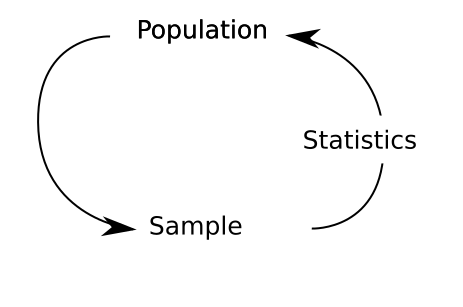
\includegraphics[width=5cm]{Images/stats.png}
\end{figure}
$Outcome_i=(Model_i)+error_i$
\end{center}
\begin{itemize}
\item we collect data on a \underline{\textit{sample}} from a much larger \underline{\textit{population}}. \underline{\textit{Statistics}} lets us to make inferences about the population from which it was derived
\item we try to predict the outcome given a model fitted to the data
\end{itemize}
\end{frame}

\begin{frame}
\frametitle{Differential gene expression}
\begin{flushright}
$t=\frac{x_1-x_2}{s_p\sqrt{\frac{1}{n_1}+\frac{1}{n_2}}}$
\end{flushright}
\begin{knitrout}
\definecolor{shadecolor}{rgb}{0.969, 0.969, 0.969}\color{fgcolor}
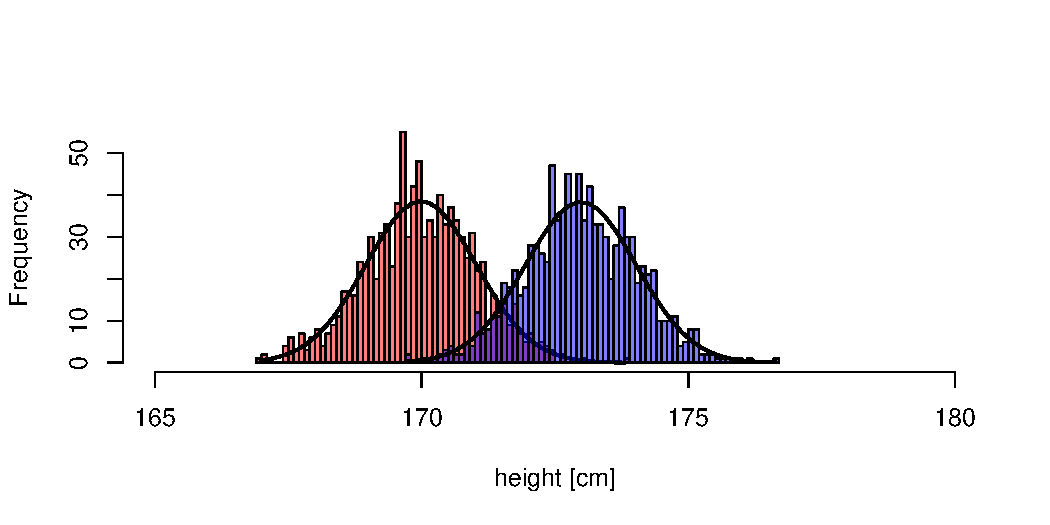
\includegraphics[width=\maxwidth]{figure/ttest-1} 

\end{knitrout}
\end{frame}


\begin{frame}
\frametitle{Differential gene expression}
\begin{block}{Simple recipe}
\begin{itemize}
\item model e.g. gene expression with random error
\item fit model to the data and/or data to the model, estimate model parameters
\item use model for prediction and/or inference
\end{itemize}
\end{block}
\begin{block}{Implications}
\begin{itemize}
\item the better model fits to the data the better statistics
\end{itemize}
\end{block}
\end{frame}




% % CM: Mast 2
% \begin{frame}
% \frametitle{The key: MAST (again)}
% \begin{itemize}
%   \item uses \underline{generalized linear hurdle model}
%   \item designed to account for stochastic dropouts and bimodal expression distribution in which expression is either strongly non-zero or non-detectable
%   \item The rate of expression \textbf{\textit{Z}}, and the level of expression \textbf{\textit{Y}}, are modeled for each gene \textbf{\textit{g}}, indicating whether gene \textbf{\textit{g}} is expressed in cell \textbf{\textit{i}} (i.e., $Z_{ig}=0$ if $y_{ig}=0$ and $z_{ig}=1$ if $y_{ig}>0$)
%   \item A \underline{logistic regression model} for the discrete variable \textbf{\textit{Z}} and a \underline{Gaussian linear model} for the continuous variable (Y|Z=1):
%    \end{itemize}
%    \begin{center}
%     $logit (P_r(Z_{ig}=1))=X_i\beta_g^D$ \newline
%     $P_r(Y_{ig}=Y|Z_{ig}=1)=N(X_i\beta_g^C,\sigma_g^2)$, where $X_i$ is a design matrix
% \end{center}
% \begin{itemize}
% \item Model parameters are \underline{fitted} using an empirical Bayesian framework
% \item Allows for a joint estimate of nuisance and treatment effects, \underline{DE is determined using the likelihood ratio test}
% \end{itemize}
% \end{frame}
% 
% 
% % CM: SCDE 2
% \begin{frame}
% \frametitle{The key: SCDE (again)}
% \begin{itemize}
%   \item \underline{models} the read counts for each gene using a mixture of a NB, negative binomial, and a Poisson distribution 
%   \item \underline{NB distribution} models the transcripts that are amplified and detected
%   \item \underline{Poisson distribution} models the unobserved or background-level signal of transcripts that are not amplified (e.g. dropout events)
%   \item subset of robust genes is used to fit, via \underline{EM} algorithm, the parameters to the mixture of models
%   \item For DE, the posterior probability that the gene shows a fold expression difference between two conditions is computed using a \underline{Bayesian approach}
% \end{itemize}
% \end{frame}
% 
% % CM: Monocole 2
% \begin{frame}
% \frametitle{The key: Monocole (again)}
% \begin{itemize}
% \item Originally designed for ordering cells by progress through differentiation stages (pseudo-time)
% \item The mean expression level of each gene is \underline{modeled with a GAM}, generalized additive model, which relates one or more predictor variables to a response variable as  
% \end{itemize}
%    \begin{center}
%     $g(E(Y))=\beta_0+f_1(x_1)+f_2(x_2)+...+f_m(x_m)$ where Y is a specific gene expression level, $x_i$ are predictor variables, g is a link function, typically log function, and $f_i$ are non-parametric functions (e.g. cubic splines)
%   \end{center}
% \begin{itemize}  
% \item The observable expression level Y is then modeled using GAM, 
% \end{itemize}
% $E(Y)=s(\varphi_t(b_x, s_i))+\epsilon$ where $\varphi_t(b_x, s_i)$ is the assigned pseudo-time of a cell and $s$ is a cubic smoothing function with three degrees of freedom. The error term $\epsilon$ is normally distributed with a mean of zero
% \begin{itemize}
% \item The DE test is performed using an \underline{approx. $\chi^2$ likelihood ratio test}
% \end{itemize}
% \end{frame}
% 
% % CM: The key implications
% \begin{frame}
% \frametitle{They key: implication}
% \begin{block}{Simple recipe}
% \begin{itemize}
% \item model e.g. gene expression with random error
% \item fit model to the data and/or data to the model, estimate model parameters
% \item use model for prediction and/or inference
% \end{itemize}
% \end{block}
% \begin{block}{Implication}
% \begin{itemize}
% \item the better model \href{http://www.itl.nist.gov/div898/handbook/pmd/section4/pmd44.htm}{fits} to the data the better statistics
% \end{itemize}
% \end{block}
% \end{frame}
% 
% % CM: Distributions
% \begin{frame}
% <<dist, echo=FALSE, fig.height=4>>=
% set.seed(1)
% par(mfrow=c(1,3))
% hist(rnbinom(1000, mu=10, size=100), col="grey50", xlab="Read Counts", main="Negative Binomial")
% d = 0.5;
% counts <- rnbinom(1000, mu=10, size=100);
% counts[runif(1000) < d] = 0;
% hist(counts, col="grey50", xlab="Read Counts", main="Zero-inflated NB");
% a = 0.1
% b = 0.1
% g = 100
% lambdas = rbeta(1000, a, b)
% counts = sapply(g*lambdas, function(l) {rpois(1, lambda=l)})
% hist(counts, col="grey50", xlab="Read Counts", main="Poisson-Beta")
% 
% @
% \end{frame}
% 
% \section{Performance}
% \begin{frame}
% \begin{center}
% \insertsection
% \end{center}
% \end{frame}
% 
% % P: no golden standard
% \begin{frame}
% \frametitle{No golden standard}
% There is no golden standard, no single best solution
% \newline
% \newline
% ...so what do we do?
% \newline
% \newline
% \begin{flushright}
% \pause we gather as much evidence as possible
% \end{flushright}
% \end{frame}
% 
% % P: assess data and distributions
% \begin{frame}
% \frametitle{Get to know your data \& wisely choose DE methods}
% Example data: 46,078 genes x 96 cells \newline
% 22,229 genes with no expression at all
% 
% <<knowdata, echo=FALSE, fig.height=4>>=
%  load("../Scripts/testData.RData")
%  idx.0 <- apply(data.counts, 1, sum)
%  idx.00 <- which(idx.0==0)
%  
%  data.counts <- as.matrix(data.counts)
%  data.subset <- as.matrix(data.counts[-idx.00,])
%  m.dummy <- matrix(data=0, nrow=nrow(data.subset), ncol=ncol(data.subset))
%  m.dummy[data.subset==0]=1
%  m.summary <- apply(m.dummy, 1, sum)
%  
%  par(mfrow=c(1,2))
%  hist(data.subset[1:200,], main="", xlab="Read Counts")
%  hist(m.summary, main="", xlab="0 counts")
% @
% \end{frame}
% 
% % P: Dal Molin
% \begin{frame}
% \frametitle{Learn from methodological papers and/or past studies}
% e.g. \href{https://www.frontiersin.org/articles/10.3389/fgene.2017.00062/full(}{Dal Molin, Barruzo and Di Camilillo, frontiers in Genetics 2017, Single-Cell RNA-Sequencing: Assessment of Differential Expression Analysis Methods}
% \begin{itemize}
% \item 10,000 genes simulated for 2 conditions with sample size of 100 cells each
% \item 8,000 genes were simulated as not differentially expressed using the same distribution (unimodal: NB and bimodal: two-component NB mixture)
% \item 2,000 genes were simulated as differentially expressed according to four types of differential expressions 
% \item real dataset: 44 mouse Embryonic Stem Cells and 44 Embryonic Fibroblsts for positive control
% \item real dataset: 80 single cells as negative control
% \end{itemize}
% \end{frame}
% 
% % P: Dal Molin plots
% \begin{frame}
% \frametitle{Learn from methodological papers and/or past studies}
% \begin{center}
% \begin{figure}
% 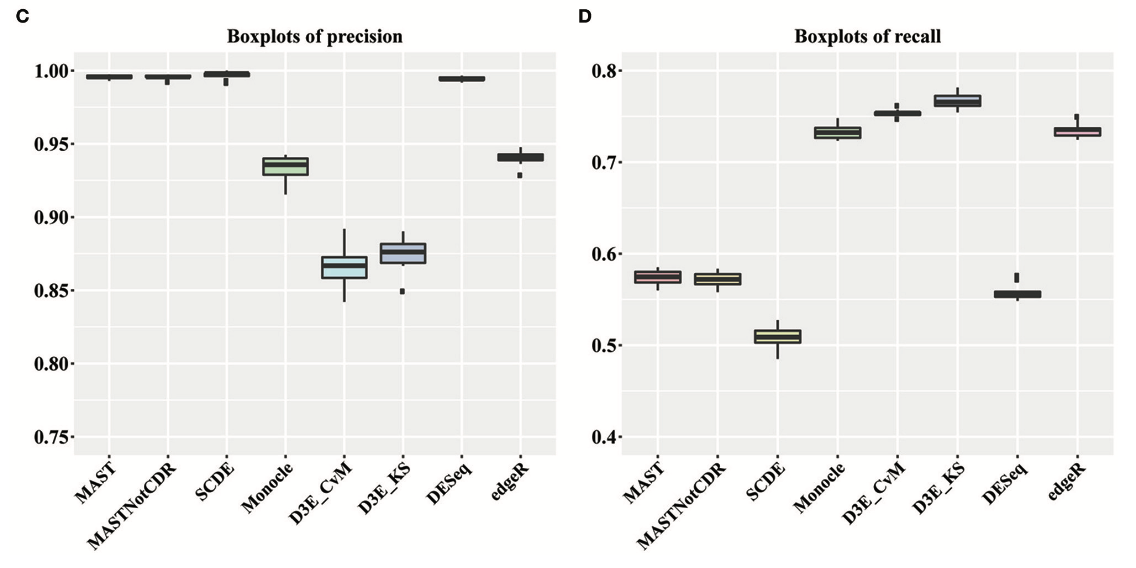
\includegraphics[width=12cm]{Images/DalMolin_fig2cd.png}
% \end{figure}
% \end{center}
% \end{frame}
% 
% % P: Miao
% \begin{frame}
% \frametitle{Compare methods}
% e.g. \href{Differential expression analyses for single-cell RNA-Seq: old questions on n???}{Miao and Zhang, Quantitative Biology 2016,4: Differential expression analyses for single-cell RNA-Seq: old questions on new data}
% \begin{center}
% \begin{figure}
% 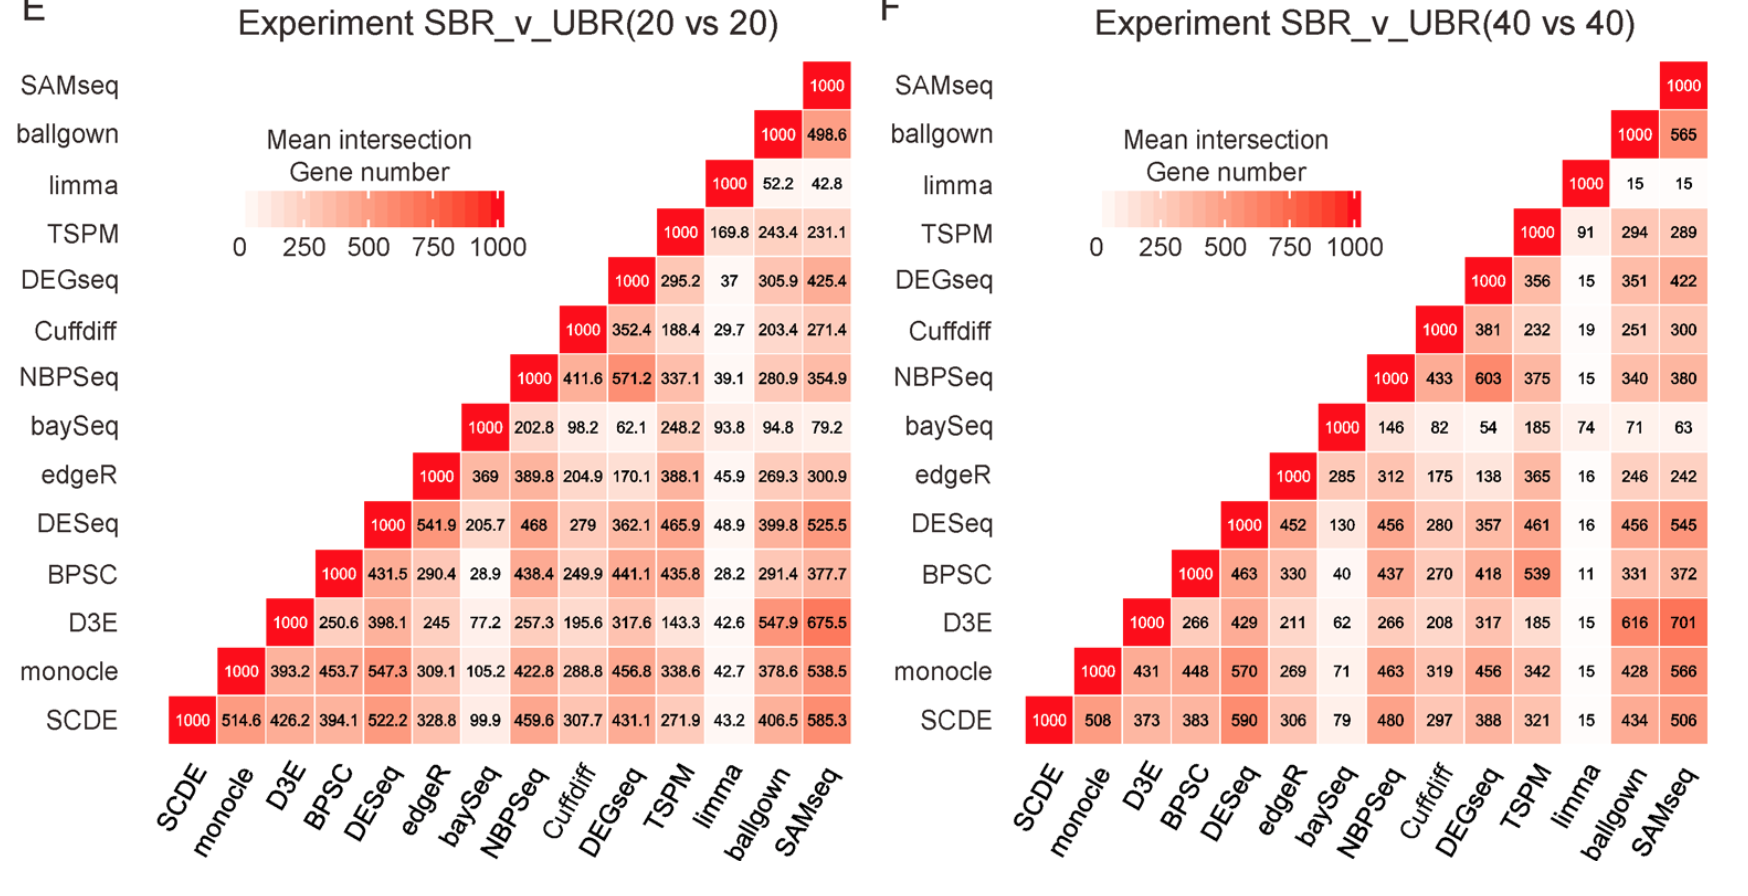
\includegraphics[width=11cm]{Images/Miao_fig1ef.png}
% \end{figure}
% \end{center}
% \end{frame}
% 
% % P: Stay critical
% \begin{frame}
% \frametitle{Stay critical}
% \begin{center}
% \begin{figure}
% 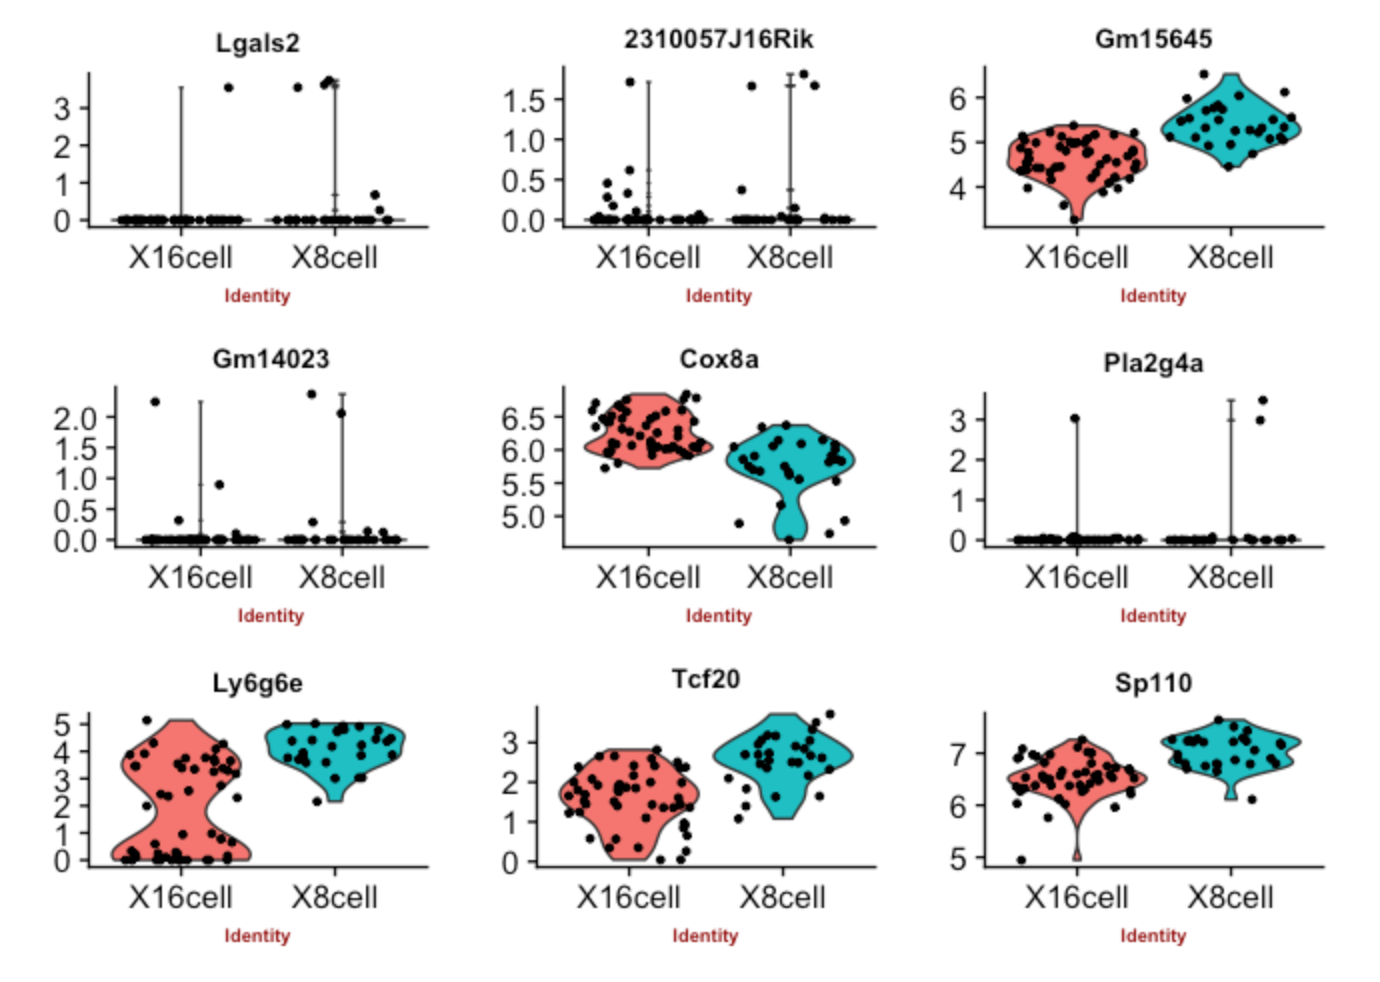
\includegraphics[width=11cm]{Images/asa1.png}
% \end{figure}
% \end{center}
% \end{frame}
% 
% % Summary section
% \section{Summary}
% \begin{frame}
% \begin{center}
% \insertsection
% \end{center}
% \end{frame}
% 
% % Summary points
% \begin{frame}
% \begin{block}{Summary}
% \begin{itemize}
% \item scRNA-seq is a rapidly growing field
% \item DE is a common task so many newer and better methods will be developed
% \item think like a statistician: get to know your data, think about distributions and models best for your data. Avoid applying methods blindly
% \item comparing methods is good as long as you are aware what you are comparing and why
% \item stay critical
% \end{itemize}
% \end{block}
% \end{frame}
% 
% % Tutorial
% \section{DE tutorial}
% \begin{frame}
% \begin{center}
% \insertsection
% \end{center}
% \end{frame}
% 
% % Tutorial points
% \begin{frame}
% \begin{block}{DE tutorial}
% Based on the dataset used is single-cell RNA-seq data (SmartSeq) from mouse embryonic development from Deng. et al. Science 2014, Vol. 343 no. 6167 pp. 193-196, "Single-Cell RNA-Seq Reveals Dynamic, Random Monoallelic Gene Expression in Mammalian Cells".
% \begin{itemize}
% \item check for differentially expressed genes between 8-cell and 16-cell stage embryos
% \item with many methods incl. SCDE, MAST, SC3 package, Pagoda, Seurat
% \item and compare the results, trying to decide on the best DE method for the dataset
% \end{itemize}
% \end{block}
% \end{frame}
% 
% \section{Finally}
% \begin{frame}
% \begin{center}
% Thank you for attention
% \newline
% \newline
% Questions?
% \newline
% \newline
% Enjoy the rest of the course
% \newline
% \newline
% olga.dethlefsen@nbis.se
% \end{center}
% \end{frame}


\end{document}
